\chapter{Testing von EGroupware mit Playwright}

Nach erfolgreicher Installation von EGroupware kann das System nun über jeden Browser aufgerufen werden und kann daher getestet werden.
Dabei wird das System mithilfe von Playwright getestet.

\section{Aufsetzen der Testumgebung}

Für das entwickeln der Tests wird die Entwicklungsumgebung Visual Studio Code verwendet da es durch die Erweiterung "Playwright Test for VSCode" von Microsoft eine sehr gute Integration der Playwright API bietet.
Mit dieser Erweiterung kann auch die vollständige Installation von Playwright in dem aktuellen Projektordner direkt in der Entwicklungsumgebung durchgeführt werden.
Dabei können die gewünschten Browser Chromium, Firefox und WebKit ausgewählt und zum Testen installiert werden.
Für diese Studienarbeit werden alle Tests in einem Chromium Browser ausgeführt.
Bei der Installation wird ein Beispieltest erstellt welcher als Vorlage für weitere Tests genutzt werden kann.
\\
\\
Für das Testen der meisten Funktionen der EGroupware Anwendung wird der Administrator Account genutzt, der automatisch bei der Installation erstellt wird.
Diesem Administrator Account wird eine E-Mail-Adresse über IMAP hinzugefügt, damit über ihn auch die E-Mail Funktion getestet werden kann.
Um diesen Account in den Tests zu nutzen wird der Nutzername und das Passwort des Administrators in der Testdatei als statisches Objekt gespeichert und kann dann in den Tests genutzt werden.

\subsection{Playwright Codegen}

Die Basis für fast alle Tests in dieser Studienarbeit wurde mithilfe von Playwright Codegen erstellt.
Dabei wird über einen Konsolenbefehl ein neuer Browser geöffnet, in dem die Interaktionen des Nutzers als Playwright Code aufgezeichnet werden.
So können große Teile des Codes für die Tests automatisch generiert werden und müssen nur noch an spezifische Anforderungen angepasst werden.
\begin{figure}[H]
    \centering
    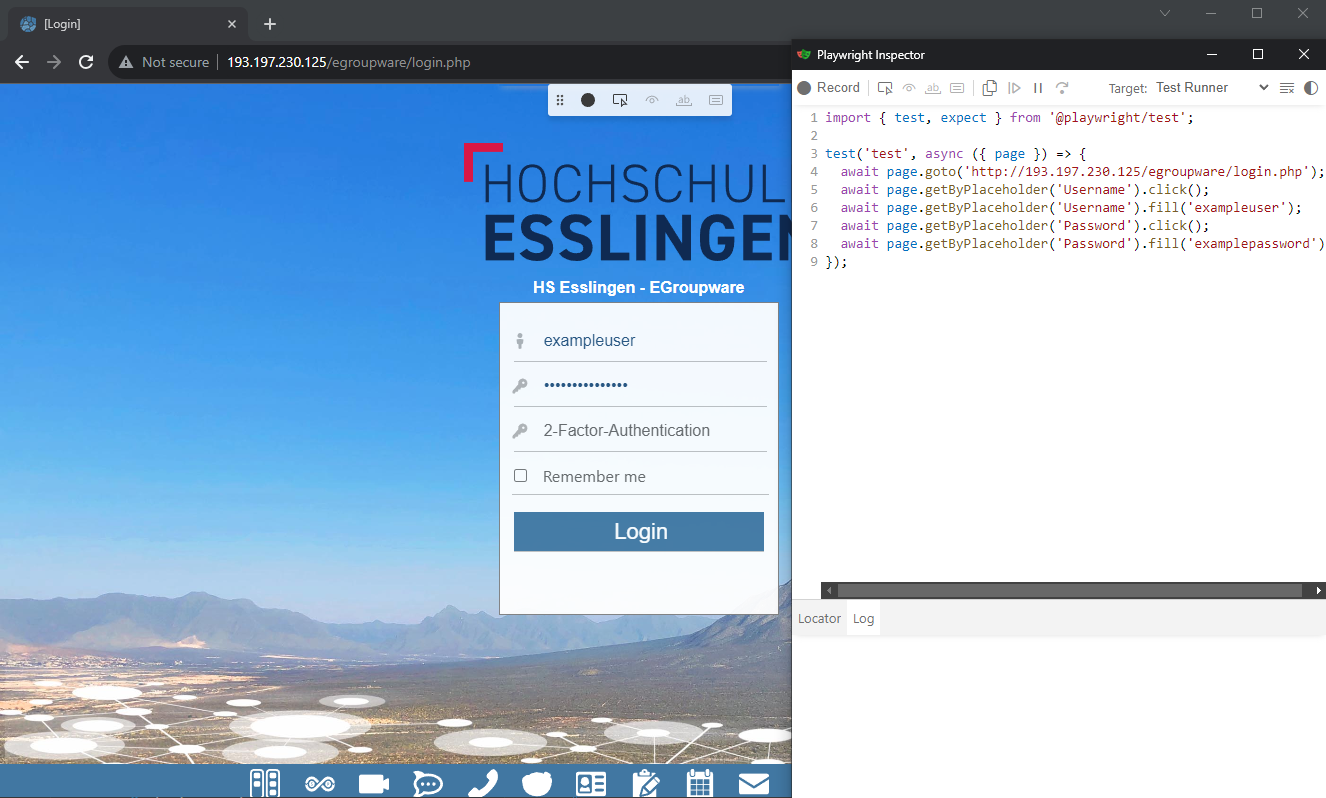
\includegraphics[width=1\textwidth]{images/Playwright_Codegen.png}
    \caption{Playwright Codegen generierter Code für das Ausfüllen eines Login Formulars}
    \label{fig:playwright-codegen}
\end{figure}
Das Tool funktioniert besonders gut für einfache Interaktionen, wie beispielsweise das Ausfüllen einfacher Formulare wie in Abbildung \ref{fig:playwright-codegen} mit einfachen User-Interface-Elementen (UI-Elementen) wie Buttons, Textfeldern und Links geeignet.
Für komplexere Interaktionen mit UI-Elementen wie beispielsweise Datepicker, welche das Auswählen eines Datums über mehrere verschachtelte Interaktionen erfordern, ist die Aufnahme-Funktion des Tools weniger geeignet.
Daher mussten Teile der Tests für das Erstellen eines Termins und das Löschen eines Nutzers manuell geschrieben werden.

\begin{figure}[H]
    \centering
    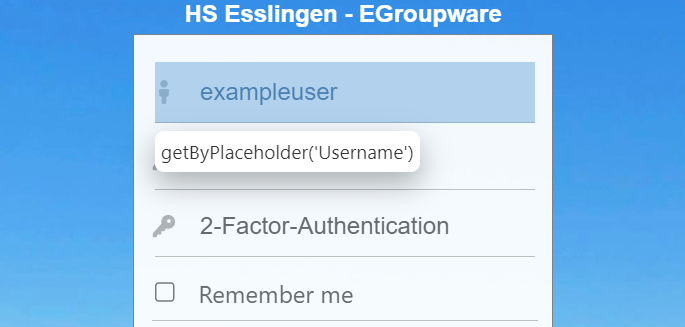
\includegraphics[width=0.5\textwidth]{images/Playwright_PickLocator.png}
    \caption{Playwright Pick Locator Funktion zum Generieren von Selektoren für UI-Elemente}
    \label{fig:playwright-pick-locator}
\end{figure}

Zu der Aufnahme-Funktion des Tools gibt es noch eine weitere Funktion, die ähnlich wie Inspect Element in Browsern funktioniert und wie in Abbildung \ref{fig:playwright-pick-locator} den Selektor für ein UI-Element generiert.
Diese Funktion kann dann für das Erstellen der manuellen Teile der Tests genutzt werden, um schnell Selektoren für UI-Elemente zu generieren.



\section{Implementierung der Tests}

Alle Tests werden in TypeScript geschrieben und können daher direkt in der Entwicklungsumgebung ausgeführt werden.
Dabei werden alle Tests in dieser Studienarbeit in einem Chromium Browser ausgeführt.
\\
Im Folgenden werden die einzelnen Tests, deren Implementierung und Deckungsbereiche näher erläutert.

\subsection{Login}

Da alle Tests der Anwendung einen eingeloggten Nutzer benötigen wird zuerst ein Login Test implementiert, der ein Nutzerobjekt mit Nutzernamen und Passwort erhält und sich dann versucht in der Anwendung einzuloggen.
Dieser Test wird zu Beginn jedes anderen Tests ausgeführt um den Nutzer einzuloggen.

\subsection{Aufrufen einer E-Mail}

Bei diesem Test wird die E-Mail Funktion der Anwendung getestet.
Der Test versucht sich als der Administrator, dessen Account einen E-Mail-Account über IMAP bekommen hat, einzuloggen und ruft dann die erste E-Mail in der E-Mail Liste auf.
Dabei wird die Verbindung der Groupware zum IMAP Server getestet.

\subsection{Erstellen eines Termins}

Beim Test zum Erstellen eines Termins wird sich als Administrator eingeloggt und dann ein Termin erstellt.
Die Daten für diesen Termin sind ähnlich wie die Daten für den Login mit dem Administrator Account in einem Objekt gespeichert und können so einfach in den Test eingefügt werden.
Jedoch wird dieses Objekt erst beim Ausführen des Tests erstellt, da das Datum für den Termin immer das aktuelle Datum sein soll und daher nicht statisch in einem globalen Objekt gespeichert werden kann.
Dafür wird mithilfe des Timestamp der Funktion Date.now() ein Datum erstellt, welches dann in einen String umgewandelt wird und in das Objekt gespeichert wird.
So kann jederzeit ein Termin erstellt werden, welcher 30 Minuten nach der Ausführung des Tests stattfindet.

\subsection{Erstellen und Löschen eines neuen Nutzers}

Der letzte Test der in dieser Studienarbeit implementiert wurde, ist eine Serie aus Tests, die die Funktionalität des Nutzermanagements abdecken sollen.
Zunächst wird mit dem Administrator Account ein neuer Nutzer erstellt, dessen Nutzerdaten in einem statischen Objekt gespeichert sind.
Ist das Erstellen des Nutzers erfolgreich, startet ein weiterer Test, der sich mit den Zugangsdaten des neuen Nutzers versucht einzuloggen.
So wird sichergestellt, dass der Nutzer erfolgreich erstellt wurde und nicht nur in der lokalen Instanz des Administrators existiert.
Ist das Einloggen mit dem Testnutzer erfolgreich, wird ein weiterer Test gestartet, der den Nutzer mit dem Administrator Account wieder löscht.
So kann der Test mit demselben Testnutzer beliebig oft ausgeführt werden, ohne dass es zu Problemen mit bereits existierenden Nutzern kommt.

\section{Ausführen der Tests}

